%Copyright 2019 Christopher M. Jermaine (cmj4@rice.edu) and Risa B. Myers (rbm2@rice.edu)
%
%Licensed under the Apache License, Version 2.0 (the "License");
%you may not use this file except in compliance with the License.
%You may obtain a copy of the License at
%
%    https://www.apache.org/licenses/LICENSE-2.0
%
%Unless required by applicable law or agreed to in writing, software
%distributed under the License is distributed on an "AS IS" BASIS,
%WITHOUT WARRANTIES OR CONDITIONS OF ANY KIND, either express or implied.
%See the License for the specific language governing permissions and
%limitations under the License.
%===============================================================
\documentclass[aspectratio=169]{beamer}
\mode<presentation> 
{
\usetheme[noshadow, minimal,numbers,riceb,nonav]{Rice}
\usefonttheme[onlymath]{serif}
\setbeamercovered{transparent}
}
\useinnertheme{rectangles}

\usepackage[english]{babel}

\usepackage{mathptmx}
\usepackage{helvet}
\usepackage{courier}
\usepackage[T1]{fontenc}
\usepackage{trajan}
\usepackage{ textcomp }
\usepackage{listings}

\newenvironment{noindentitemize}
{ \begin{itemize}
 \setlength{\itemsep}{1.5ex}
  \setlength{\parsep}{0pt}   
  \setlength{\parskip}{0pt}
 \addtolength{\leftskip}{-2em}
 }
{ \end{itemize} }

\newenvironment{noindentitemize2}
{ \begin{itemize}
  \setlength{\itemsep}{0ex}
  \setlength{\parskip}{0pt}
  \setlength{\parsep}{0pt}   
  \addtolength{\leftskip}{-2em}  }
{ \end{itemize} }



\lstnewenvironment{SQL}
  {\lstset{
        aboveskip=5pt,
        belowskip=5pt,
        escapechar=!,
        mathescape=true,
        upquote=true,
        language=SQL,
        basicstyle=\linespread{0.94}\ttfamily\footnotesize,
        morekeywords={PRINT, CURSOR, OPEN, FETCH, CLOSE, DECLARE, BEGIN, END, PROCEDURE, FOR, EACH, WITH, PARTITION, 	TEST, WHETHER, PROBABILITY, OUT,LOOP,IF,CONTINUE, HANDLER,CALL, FUNCTION, RETURNS, LANGUAGE,BODY,RETURN, REPLACE,plpgsql,
        RAISE, NOTICE,
        REPLACE, ROW, BEFORE, EXIT, TEXT, REFCURSOR, QUOTE_LITERAL, DELIMITER,CONCAT,FOUND,LEAVE },
        deletekeywords={VALUE, PRIOR},
        showstringspaces=true}
        \vspace{0pt}%
        \noindent\minipage{0.65\textwidth}}
  {\endminipage\vspace{0pt}}
  
  
\lstnewenvironment{SQLtiny}
  {\lstset{
        aboveskip=5pt,
        belowskip=5pt,
        escapechar=!,
        mathescape=true,
        upquote=true,
        language=SQL,
        basicstyle=\linespread{0.94}\ttfamily\tiny,
        morekeywords={PRINT, CURSOR, OPEN, FETCH, CLOSE, DECLARE, BEGIN, END, PROCEDURE, FOR, EACH, WITH, PARTITION, 	TEST, WHETHER, PROBABILITY, OUT,LOOP,IF,CONTINUE, HANDLER,CALL, FUNCTION, RETURNS, LANGUAGE,BODY,RETURN, REPLACE,plpgsql,
        RAISE, NOTICE,
        REPLACE, ROW, BEFORE, EXIT, TEXT, REFCURSOR, QUOTE_LITERAL, DELIMITER,CONCAT,FOUND,LEAVE },
       deletekeywords={VALUE, PRIOR},
        showstringspaces=true}
        \vspace{0pt}%
        \noindent\minipage{0.47\textwidth}}
  {\endminipage\vspace{0pt}}

%===============================================================%

\title[]
{Tools \& Models for Data Science}

\subtitle{Introduction to Modeling 1}

\author[]{Chris Jermaine \& Risa Myers}
\institute
{
  Rice University 
}

\date[]{}

\subject{Beamer}


\begin{document}

\begin{frame}
 \titlepage
\end{frame}

%***********************************************************
\begin{frame}{What is a Model?}

\begin{itemize}
\item Many definitions!
\item Traditional statistical definition:
	\begin{itemize}
	\item A set of assumptions regarding the (stochastic) process that generated the data
	\item Classical statistical approach: 
		\begin{itemize}
		\item Assume some stochastic process \footnote {  A stochastic process is a random process that changes over time i.e., a mathematical object usually defined as a collection of random variables
} generated the data
		\item We want to figure out how the model generated the data
		\end{itemize}
	\end{itemize}
\item More modern definition:
	\begin{itemize}
	\item A mathematical object that enables an analyst to use data to understand the past and present,
	and make predictions about the future
	\end{itemize}
\end{itemize}
\end{frame}
%***********************************************************
\begin{frame}{Why Do We Model?}

\begin{itemize}
\item Real data are big, complex, difficult to understand
\item A model is (hopefully!) compact, simple, comprehensible
\item Modeling is all about simplification
\end{itemize}
\end{frame}
%***********************************************************
\begin{frame}{Why Do We Model?}

\begin{itemize}
\item Real data are big, complex, difficult to understand
\item A model is (hopefully!) compact, simple, comprehensible
\end{itemize}

\begin{itemize}
\item Just as important:
\begin{itemize}
	\item Models can often be used to make predictions about future events
	\item Example: Supervised learning
\end{itemize}
\end{itemize}
\end{frame}
%***********************************************************
\begin{frame}{Modeling Process}

\begin{itemize}
\item This what data scientists do every day
\item In modeling, four big tasks
	\begin{itemize}
	\item 1. Choosing the model---choose family, complexity, hyperparameters
	\item 2. Learning the model---``fit'' model to data by adjusting parameters
	\item 3. Validating the model---make sure model matches data
	\item 4. Applying the model---use the model to explain past/present make predictions on future
	\end{itemize}
\item Often, 1 thru 3 repeated iteratively until model matches data
\item Will focus on all four in upcoming weeks!
\end{itemize}
\end{frame}
%***********************************************************
\begin{frame}{1. Choosing the model}

\begin{itemize}
\item Select the distribution or distribution family \footnote{Probability distributions are not a single distribution or function, but are a family of distributions because they have different shape parameters that allow them to have a variety of different forms/shapes.}: e.g. Exponential family
\item Choosing the hyperparameters \footnote{A hyperparameter is a parameter of a prior distribution used in a model
}
\begin{itemize}
\item Can be informative (e.g. biasing a parameter to be close to 0)
\item Can be noninformative (e.g. allowing values to be selected uniformly over a range)
\end{itemize}
\item Note that hyperparameters are external to the model and aren't based on the data
\item Model parameters are estimated from / learned from the data
\end{itemize}
\end{frame}
%***********************************************************
\begin{frame}{2. Learning the model}

\begin{itemize}
\item Use the existing dataset to figure out the model parameters
\item Approach can be dependent on the quantity of data you have
\item Example 
\begin{itemize}
\item Choose an appropriate loss function 
\item Minimize or maximize the loss function to optimize the parameters
\end{itemize}
\end{itemize}
\end{frame}
%***********************************************************
\begin{frame}{Course Scope}

\begin{columns}
\begin{column}{0.5\textwidth}
\begin{itemize}
\item Models can be biased based on the data you choose
\item Data evolves over time
\item These are really important issues
\item $\ldots$ that we will NOT cover in this course
\end{itemize}
\end{column}
\begin{column}{0.5\textwidth}
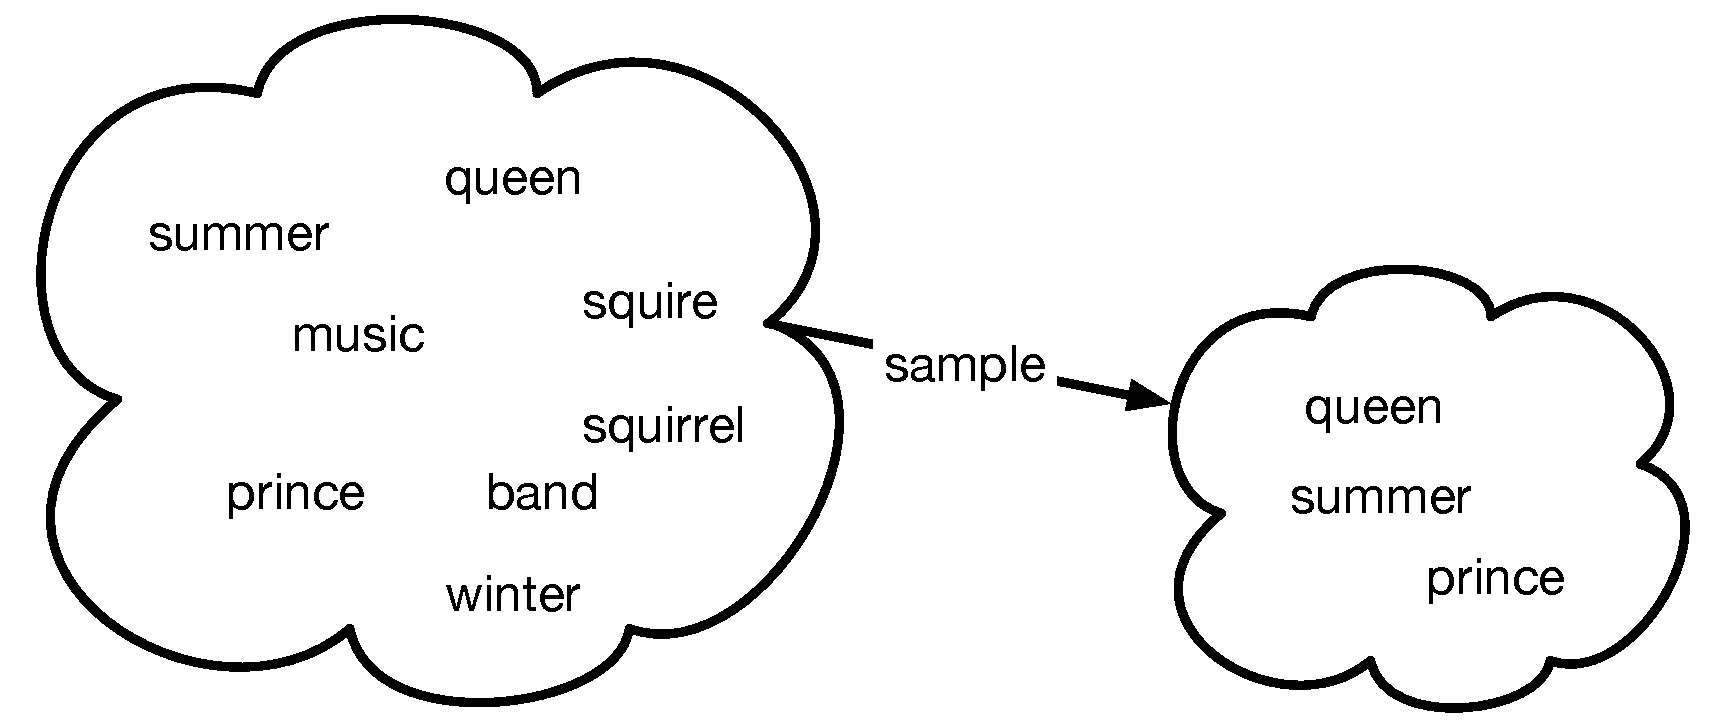
\includegraphics[width=1\textwidth]{lectModel1/populationSample.pdf}
\end{column}
\end{columns}
\end{frame}

%***********************************************************
\begin{frame}{3. Validating the model}

\begin{itemize}
\item Assume you have ``learned'' a model
\item Want to figure out if the model is useful or not
\item Common problem is Overfitting
\item Approach can be dependent on the quantity of data you have
\end{itemize}
\end{frame}
%***********************************************************
\begin{frame}{4. Applying the model}

\begin{itemize}
\item Use the model on new data
\item This is what you report \& use
\end{itemize}
\end{frame}
%***********************************************************
\begin{frame}{Statistical Modeling}

\begin{itemize}
\item Many (not all!) models rely on the idea of probability
	\begin{itemize}
		\item ``the extent to which an event is likely to occur, measured by the ratio of the favorable cases to the whole number of cases possible''
		\item Flip a coin
		\item H\hspace{1em}T\hspace{1em}H\hspace{1em}H\hspace{1em}H\hspace{1em}H
		\item P(Heads) = $\frac{5}{6}$
	\end{itemize}
\item Probability is used less in modern models
	\begin{itemize}
		\item Deep learning
	\end{itemize}

\end{itemize}
\end{frame}
%***********************************************************
\begin{frame}{Statistical Modeling}

\begin{itemize}
\item Many (not all!) models rely on the idea of probability
	\begin{itemize}
		\item ``the extent to which an event is likely to occur, measured by the ratio of the favorable cases to the whole number of cases possible''
	\end{itemize}
\item What about infinitely many possible events?
\item Then probability tends to zero
	\begin{itemize}
		\item Ex: the chance I jump exactly 3 feet
		\item Ex: the chance class ends at exactly 11AM
		\item Ex: the chance it takes 5 hours to complete A2 
	\end{itemize}
\end{itemize}
\end{frame}
%***********************************************************
\begin{frame}{Statistical Modeling}

\begin{itemize}
\item Many (not all!) models rely on the idea of probability
	\begin{itemize}
		\item ``the extent to which an event is likely to occur, measured by the ratio of the favorable cases to the whole number of cases possible''
	\end{itemize}
\item What about infinitely many possible events?
\item Then probability tends to zero
	\begin{itemize}
		\item Ex: the chance I jump exactly 3 feet
		\item Ex: the chance class ends at exactly 11A
		\item Ex: the chance it takes 5 hours to complete A2 
	\end{itemize}
\item Motivation for the idea of probability density
\end{itemize}
\end{frame}
%***********************************************************
\begin{frame}{Probability Density}

\begin{itemize}
\item Probability density gets around this problem of having to deal with very small absolute probabilities
	\begin{itemize}
	\item Measures the relative likelihood of an event---not absolute
	\end{itemize}
\item Probability A2 takes 5 hours is nonsensical
\item But...
	\begin{itemize}
	\item Probability density at  `A2 takes 5 hours' is $5X$'\ A2 takes 1 hour
	\item Sensical!
	\end{itemize}
\end{itemize}
\end{frame}
%***********************************************************

\begin{frame}{Probability Density Function}

\begin{itemize}
\item A PDF is a function that computes the relative likelihood of an event
\item Most famous: normal PDF
	$$f_{\textrm{Normal}}(x | \mu, \sigma) = \sigma^{-1} (2\pi)^{-\frac{1}{2}}
		e^{-\frac{1}{2}(x - \mu)^2\sigma^{-2}}$$
\end{itemize}
\begin{columns}
\begin{column}{0.5\textwidth}
\begin{itemize}
\item A PDF can be used to calculate the probability of a range of events
\item $\int_a^b f(x)dx$ is the probability we see a value in range $a$ to $b$
\end{itemize}
\end{column}
\begin{column}{0.5\textwidth}
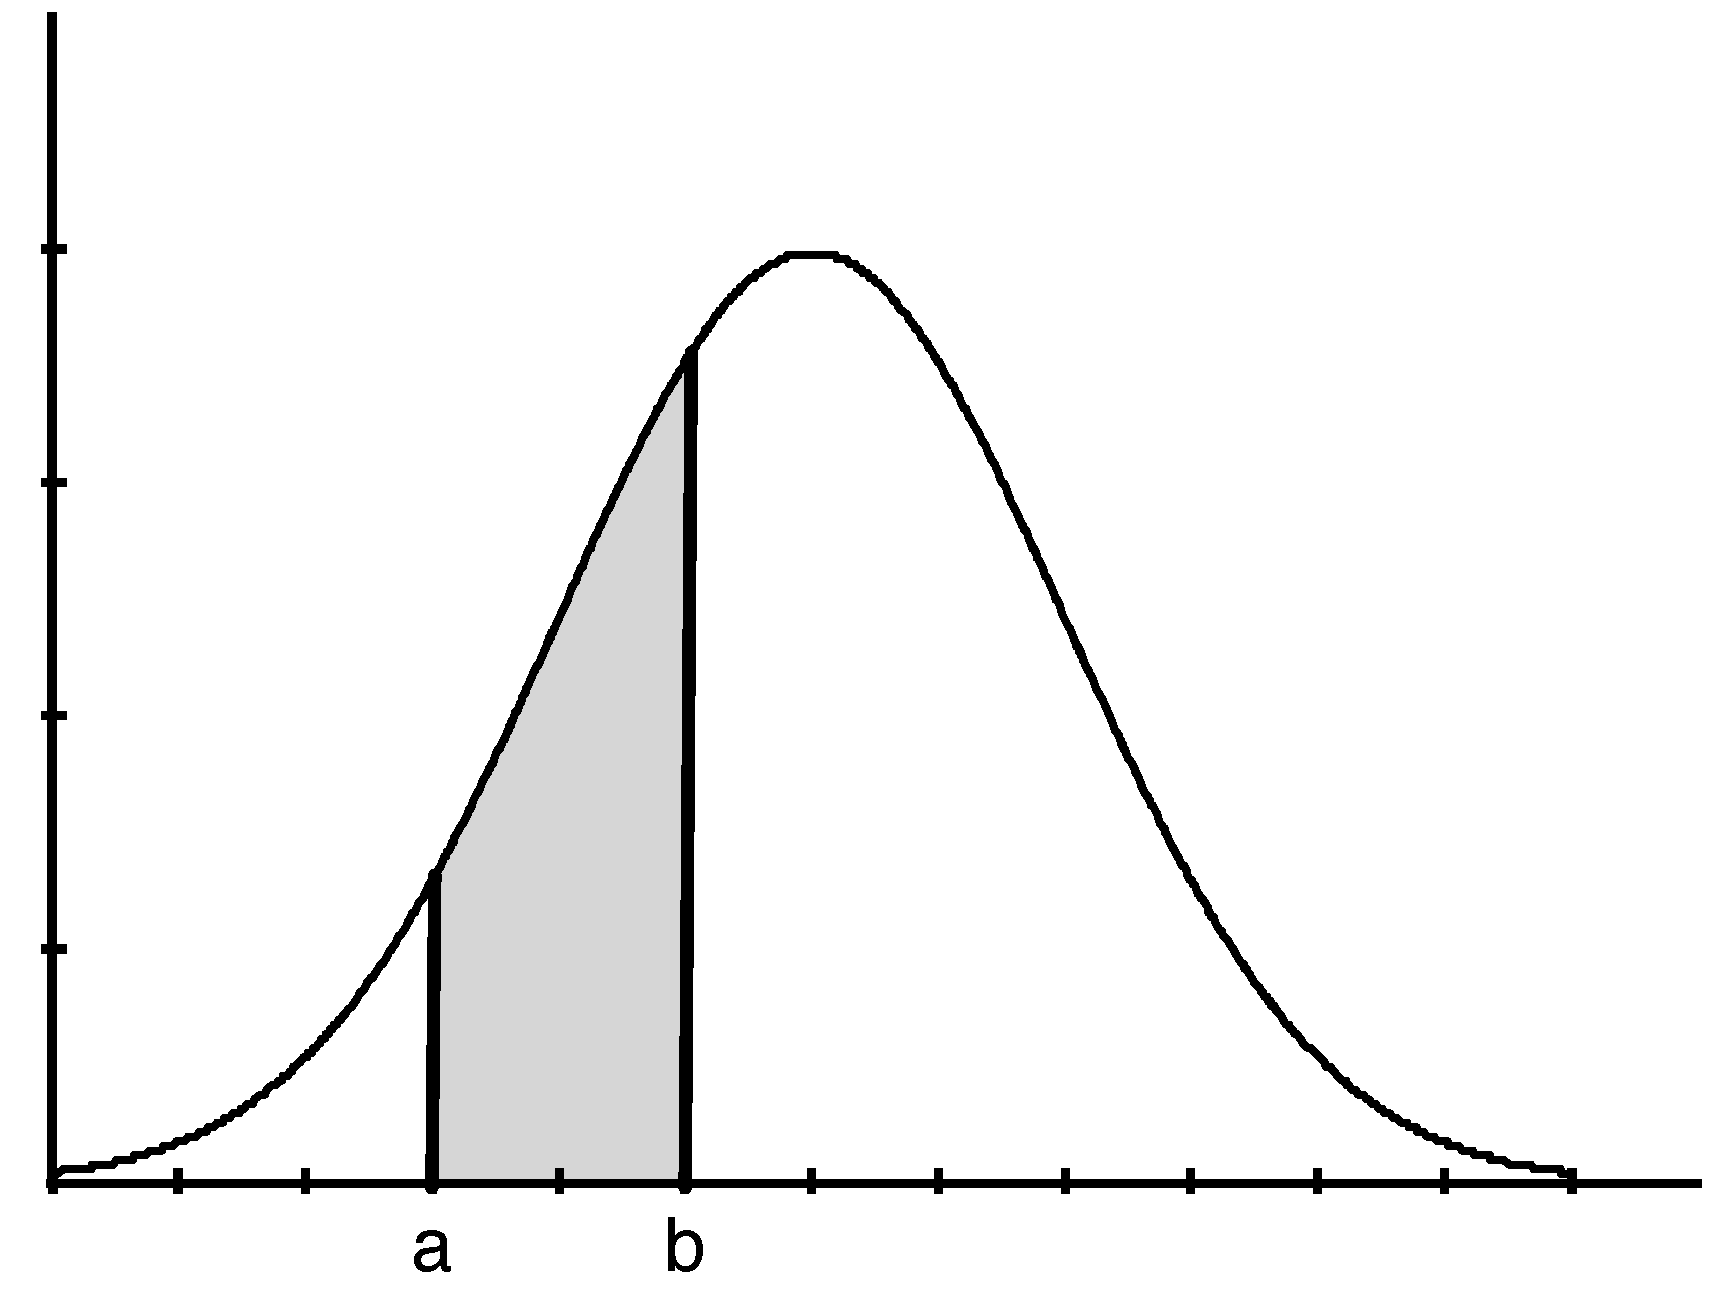
\includegraphics[width=1\textwidth]{lectModel1/normalPDFab.pdf}
\end{column}
\end{columns}
\end{frame}

%***********************************************************

\begin{frame}{The Normal/Gaussian Distribution}

\begin{columns}
\begin{column}{0.5\textwidth}
\begin{itemize}
\item Is continuous
\item Arguably the most popular statistical distribution
\item Many data in real life follow this distribution
\item Models processes that can be viewed as the sum of multiple processes
\item The math is nice: $e^a * e^b = e^{a+b}$
\item Is super important because of the Central Limit Theorem
\begin{itemize}
	\item Under certain conditions the histogram of the normalized sum of independent random variables will follow a Normal distribution
	% n > 30
\end{itemize}
\end{itemize}
\end{column}
\begin{column}{0.5\textwidth}
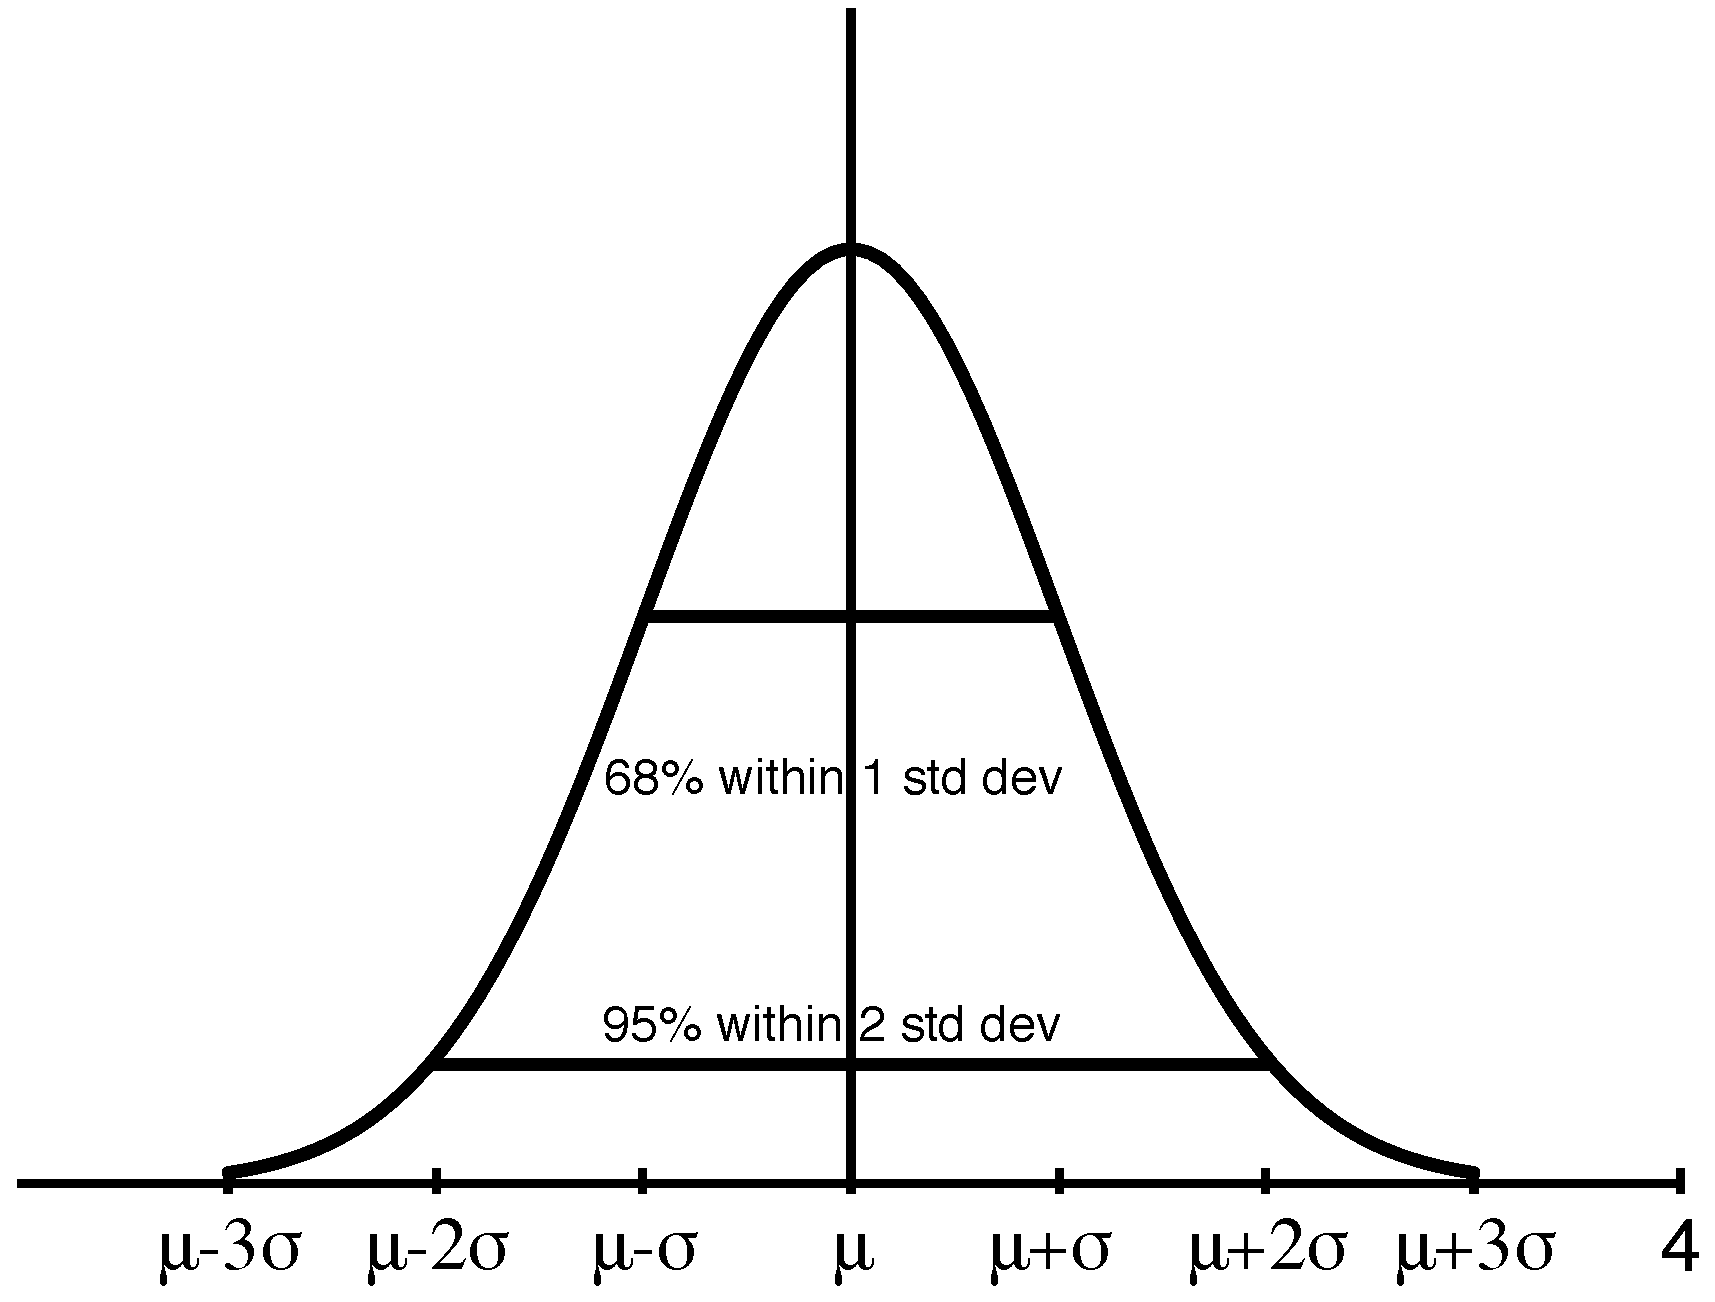
\includegraphics[width=1\textwidth]{lectModel1/normalPDF.pdf}
\begin{itemize}
\item Parameters
\begin{itemize}
\item $\mu$ = the mean value
\item $\sigma^2$ = the variance
% \mu is the center
% \sigma says something about the width of the curve
\end{itemize}
\end{itemize}

\end{column}
\end{columns}
\end{frame}

%***********************************************************

\begin{frame}{Choosing a Model}

\begin{itemize}
\item There is a well known aphorism:
	\begin{itemize}
	\item ``All models are wrong, but some are useful''
	\end{itemize}	
\item Remember:
	\begin{itemize}
	\item ``A model is (hopefully!) compact, simple, comprehensible''
	\item We choose models to reduce, simplify, comprehend data
	\item Hopefully, without incurring (too much) inaccuracy!!
	\end{itemize}
\end{itemize}
\end{frame}
%***********************************************************

\begin{frame}{Example: Predicting Grade in Class}

\begin{columns}
\begin{column}{0.7\textwidth}
\begin{itemize}
	\item A student has completed 5/10 assignments
	\begin{itemize}
	\item Want to predict grade in class
	\end{itemize}
	\item First, choose a model
	\begin{itemize}
	\item Ex: assume $X_i \sim \textrm{Normal} (\mu, \sigma)$ 
	\item $i$ is the identity of the assignment
	\item Note: $X_i$ is a random variable controlling a score
	\item $f_{X_i} (x)$ gives relative likelihood $X_i$ takes value $x$
	\item (or the probability if $X_i$ is discrete!)
	\item So $f_{X_i} (x) = f_{\textrm{Normal}}(x | \mu, \sigma)$
	\end{itemize}
\end{itemize}
\end{column}
\begin{column}{0.3\textwidth}
\begin{tabular}{|r|c|} \hline
$i$ & Score \\ \hline
1 & 89 \\ \hline
2 & 92 \\ \hline
3 & 78 \\ \hline
4 & 94 \\ \hline
5 & 88 \\ \hline
6 & -  \\ \hline
7 &  - \\ \hline
8 &  - \\ \hline
9 &  - \\ \hline
10 & - \\ \hline \hline
Avg & ? \\ \hline
\end{tabular}
\end{column}
\end{columns}
\end{frame}
%***********************************************************
\begin{frame}{Should We be Assuming Scores are Normal?}
\begin{itemize}
\item Probably not, for a single student
\item Scores are probably relatively similar for a single student
\item Sometimes life happens, and a student does poorly on an assignment
\item So, reality might be a more right skewed curve
\item Also, scores are usually discrete
\item But it's typically easier to use continuous distributions in practice
\end{itemize}
\end{frame}

%***********************************************************
\begin{frame}{Random Variables}
\begin{itemize}
\item $X_i$ is a Random Variable (RV)
\item It is normally distributed with some mean and variance, $\mu$ and $\sigma$
\item e.g. $X_2$ denotes the RV that controls the student's score on assignment 2
\item A RV is basically a machine:
\begin{enumerate}
\item Press a button
\item A stochastic process spits out an outcome
\end{enumerate}
\item The distribution of the RV controls which stochastic process is inside the machine
\end{itemize}
\end{frame}

%***********************************************************
\begin{frame}{Learning the Model}

\begin{columns}[c]
\begin{column}{0.7\textwidth}
\begin{itemize}
	\item Scores so far: $\{89, 92, 78, 94, 88\}$
	\begin{itemize}
	\item Estimate mean $\mu = 88.2$, $\sigma^2 = 30.56$
	\item[?] Where did we get these values? % the provided data  - mean and variance
\end{itemize}
	\item Thus, $X_i \sim \textrm{Normal} (\mu, \sigma^2) \sim \textrm{Normal}(88.2, 30.56)$
	\item And so ($\sum_{i=6...10} X_i) \sim \textrm{Normal} (88.2 \times 5, (30.56 \times 5))$
	\item This is an example of the ``Method of moments'' estimator
\begin{itemize}
	\item 1st: Mean
	\item 2nd: Variance
	\item $\ldots$ %3rd is skewness, 4th is Kurtosis
	\item[?] What assumptions have we made? % the data are independent
	\end{itemize}
\end{itemize}
\end{column}
\begin{column}{0.3\textwidth}
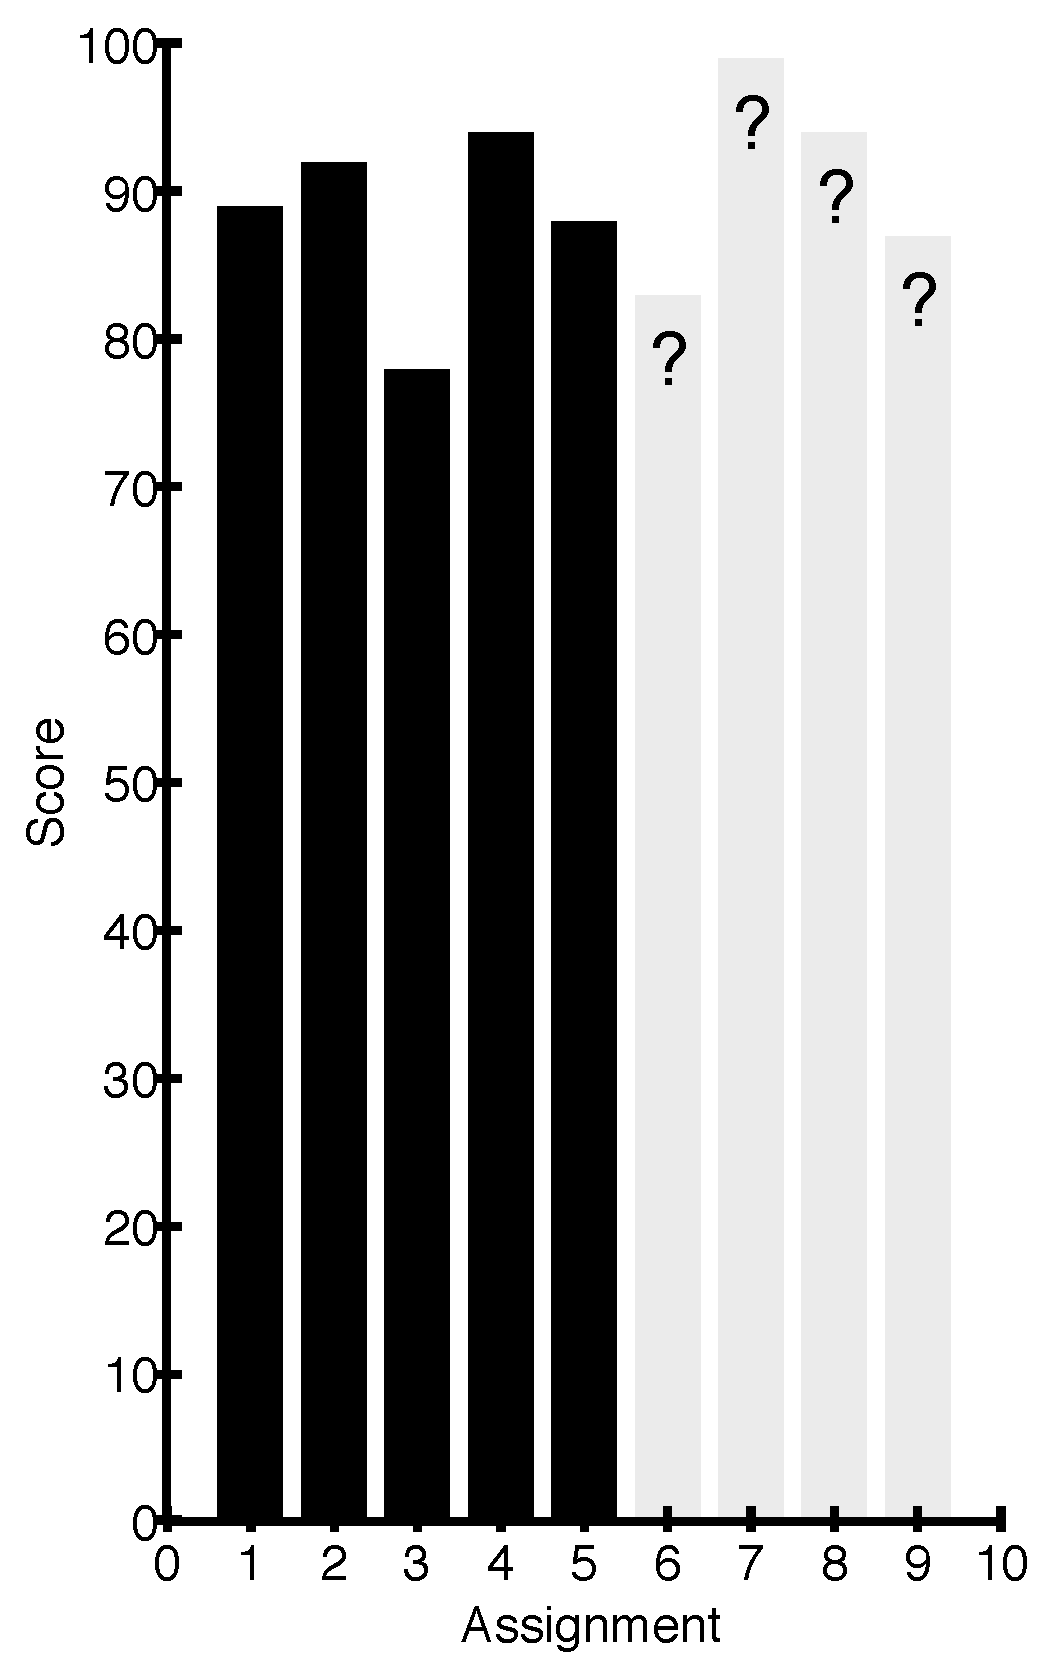
\includegraphics[width=1\textwidth]{lectModel1/scores.pdf}
\end{column}
\end{columns}
\end{frame}
%***********************************************************
\begin{frame}{Our Assumptions}

\begin{itemize}
	\item The data are independent
	\item Probably not true in this case
	\item If a student does well so far, the student is likely to do well the rest of the semester
	\item If a student is  doing poorly, the student may give up and do even worse
	\item We could take this into account (add covariances, etc.),  but not in this course
\end{itemize}
\end{frame}
%***********************************************************
\begin{frame}{Validating the Model}

\begin{itemize}
	\item So little data, won't do it here
	\begin{itemize}
	\item In general, requires checking whether $\textrm{Normal} (88.2, 30.56)$ actually describes data
	\item Often involves holding back test and validation sets
	\item More on this later
	\item Let's just assume our model is valid...
	\end{itemize}
\end{itemize}
\end{frame}
%***********************************************************
\begin{frame}{Getting Ready to Apply the Model}

\begin{itemize}
	\item Scores so far: $\{89, 92, 78, 94, 88\}$
	\begin{itemize}
	\item Estimate mean $\mu = 88.2$, $\sigma^2 = 30.56$
	\item Thus, $X_i \sim \textrm{Normal} (88.2, 30.56)$
	\item And so $\big(\sum_{i=6...10} X_i\big) \sim \textrm{Normal} (88.2 \times 5, (30.56 \times 5))$
	\end{itemize}
\end{itemize}
\end{frame}
%***********************************************************
\begin{frame}{Applying the Model}

\begin{columns}[c]
\begin{column}{0.6\textwidth}
\begin{itemize}
	\item We have a mean of 88.2 on the first 5 scores
	\item We expect a mean of 88.2 on the next 5 scores
	\item This gives us a total of $88.2 * 10 = 882$ for the expected sum on the mean of all the scores
	\item 95\% confidence on sum: $882 \pm 2 \times 12.36 = 882 \pm 24.7$
	\item[?] Where does the $\pm 2 \times 12.36$ come from? % (v*5)^0.5
=	\item Hence, 95\% confidence on grade is $88.2 \pm 2.47$
\end{itemize}
\end{column}
\begin{column}{0.4\textwidth}
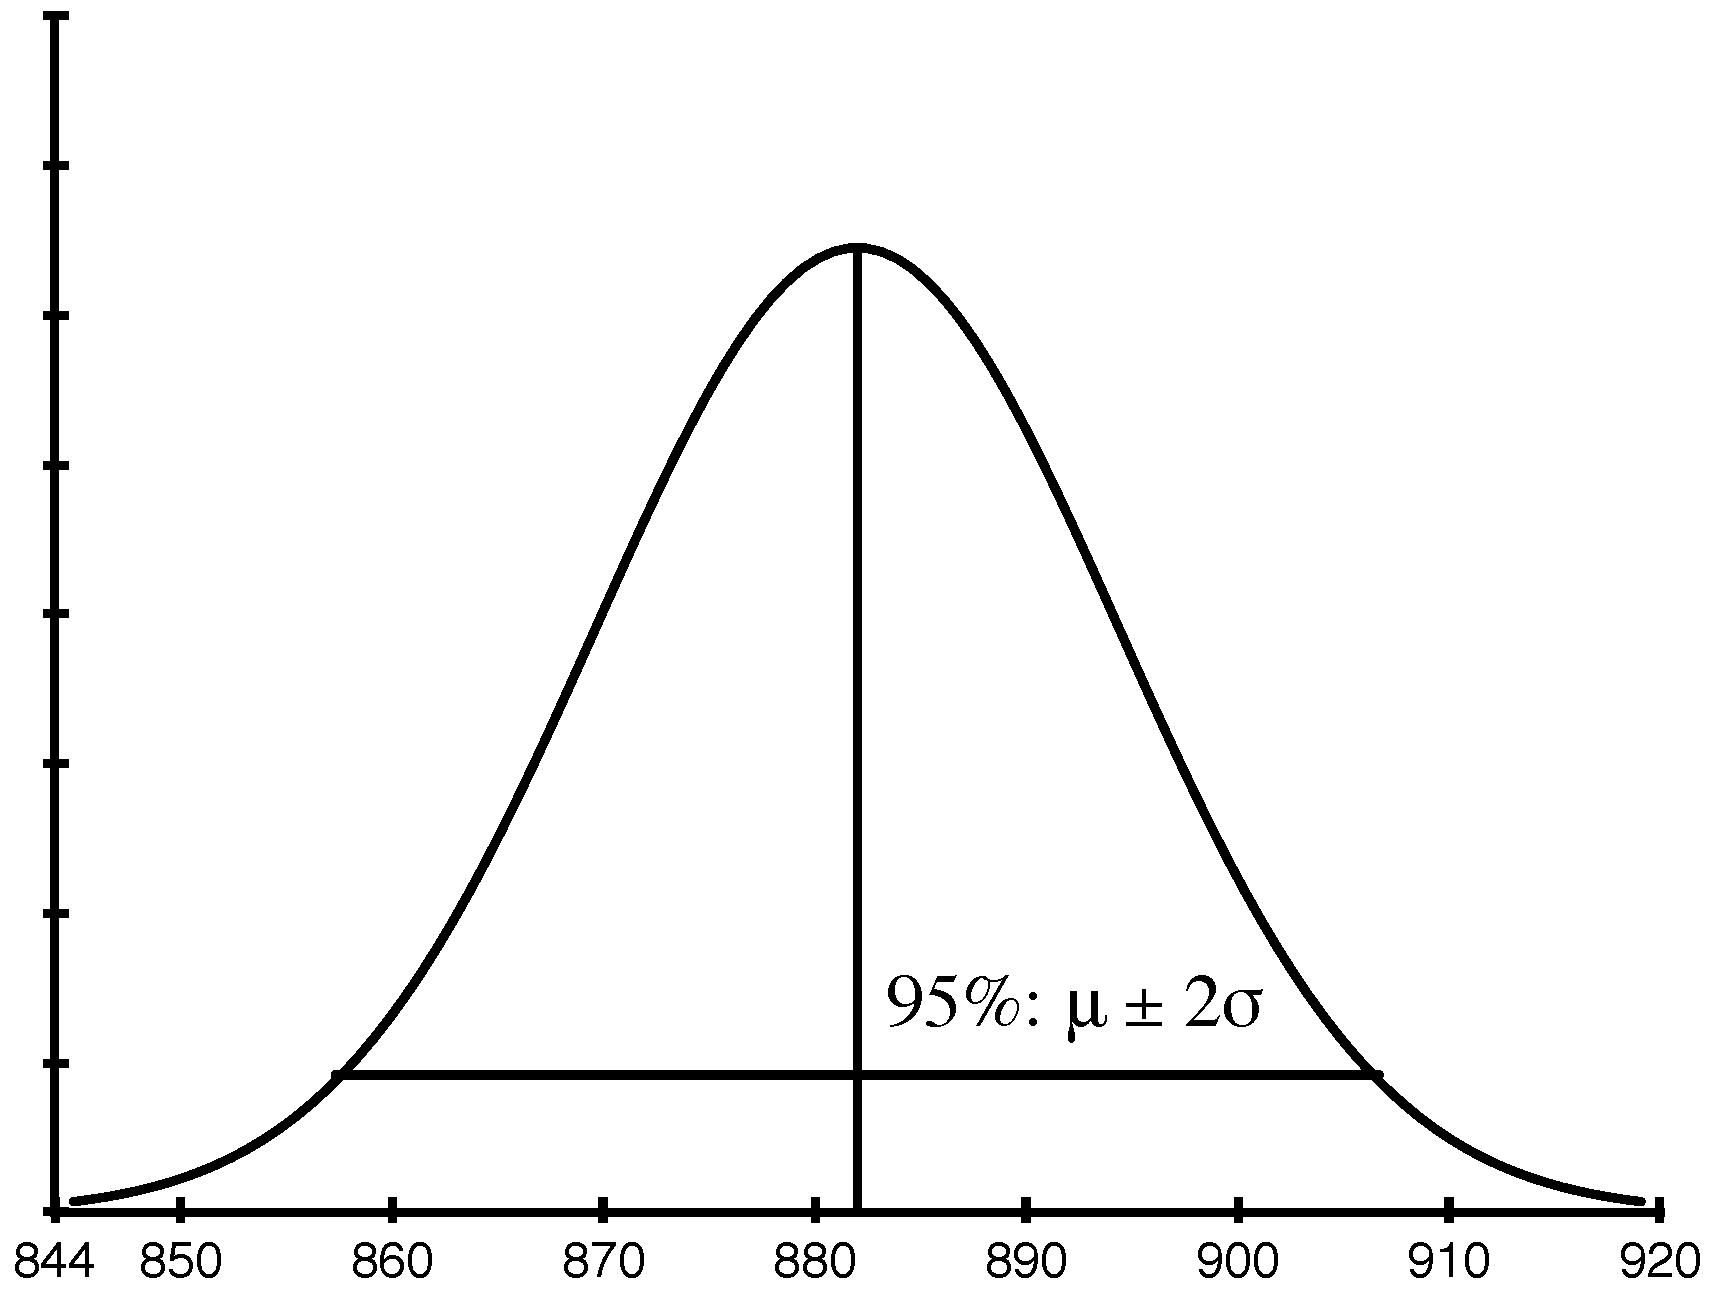
\includegraphics[width=1\textwidth]{lectModel1/normalScoresV2.pdf}
\end{column}
\end{columns}
\end{frame}
%***********************************************************
\begin{frame}{The Sniff Test}
\begin{itemize}
\item 95\% confidence interval on grade is $88.2 \pm 2.47$
\item[?] What do we mean by 95\% confidence?
\end{itemize}
\end{frame}
%***********************************************************
\begin{frame}{The Sniff Test}
\begin{itemize}
\item 95\% confidence interval on grade is $88.2 \pm 2.47$
\item What do we mean by 95\% confidence?
\begin{itemize}
\item If repeated samples were taken out of a given population, and you calculated a 95\% confidence interval for each sample, that means that 95\% of these intervals would contain the population mean
\item Remember that CIs are the probability of the parameter lying in the interval BEFORE you calculate this interval (not that the parameter has a 95\% chance of being in a given interval you've calculated with 95\% CI)
\end{itemize}
\end{itemize}
\end{frame}
%***********************************************************
\begin{frame}{The Sniff Test}
\begin{itemize}
\item 95\% confidence interval on grade is $88.2 \pm 2.47$
\item[?] Does this seem reasonable?
\end{itemize}
\end{frame}
%***********************************************************
\begin{frame}{The Sniff Test}
\begin{itemize}
\item 95\% confidence interval on grade is $88.2 \pm 2.47$
\item Does this seem reasonable?
\item The standard deviation seems low
\item Low standard deviation on existing scores implies small range in the future
\item[?] Where does the smallness come from?
\end{itemize}
\end{frame}
%***********************************************************
\begin{frame}{The Sniff Test}
\begin{itemize}
\item 95\% confidence on grade is $88.2 \pm 2.47$
\item Does this seem reasonable?
\item The standard deviation seems low
\item Low standard deviation on existing scores implies small range in the future
\item Where does the smallness come from?
\item Our standard deviation is based on only 5 data points
\item We could have a bad estimation for the moments of distribution because we have such little data
\end{itemize}
\end{frame}

%***********************************************************
\begin{frame}{Another Example: Assignment Turn In}

\begin{itemize}
	\item 5/10 students have completed the assignment
	\item 168 hours (one week) to complete the assignment
	\begin{itemize}
	\item Want to predict how many have completed by 1 hour before due date
	\end{itemize}
\end{itemize}

\end{frame}
%***********************************************************
\begin{frame}{Choosing a Model}

\begin{itemize}
	\item 5/10 students have completed the assignment
	\item 168 hours (one week) to complete the assignment
	\begin{itemize}
	\item Want to predict how many have completed by 1 hour before due date
	\item $X_i$: number of hours after assignment student $i$ turns in
	\item Assume $X_i \sim \textrm{Exponential} (\lambda)$
	\item Exponential PDF:
	$$f_{Exp} (x | \lambda) = \lambda e^{-\lambda x}$$
	\end{itemize}
\end{itemize}
\end{frame}
%***********************************************************
\begin{frame}{The Exponential Distribution}

\begin{columns}[c]
\begin{column}{0.6\textwidth}
\begin{itemize}
\item Is continuous
\item Has 1 parameter $\lambda$, which determines how quickly the mass drops off
\item Mean: $\lambda^{-1}$
\item Variance: $\lambda^{-2}$
\item Is ``memoryless''
\begin{itemize}
	\item That $t$ time units have passed doesn't matter
	\item Means if waited $t$ units so far...
	\item $f_{Exp} (x | \lambda, x \ge t) = f_{Exp} (x - t | \lambda)$
\end{itemize}
\item Good for modeling time horizons (e.g. arrivals) and time between events
\end{itemize}
\end{column}
\begin{column}{0.4\textwidth}
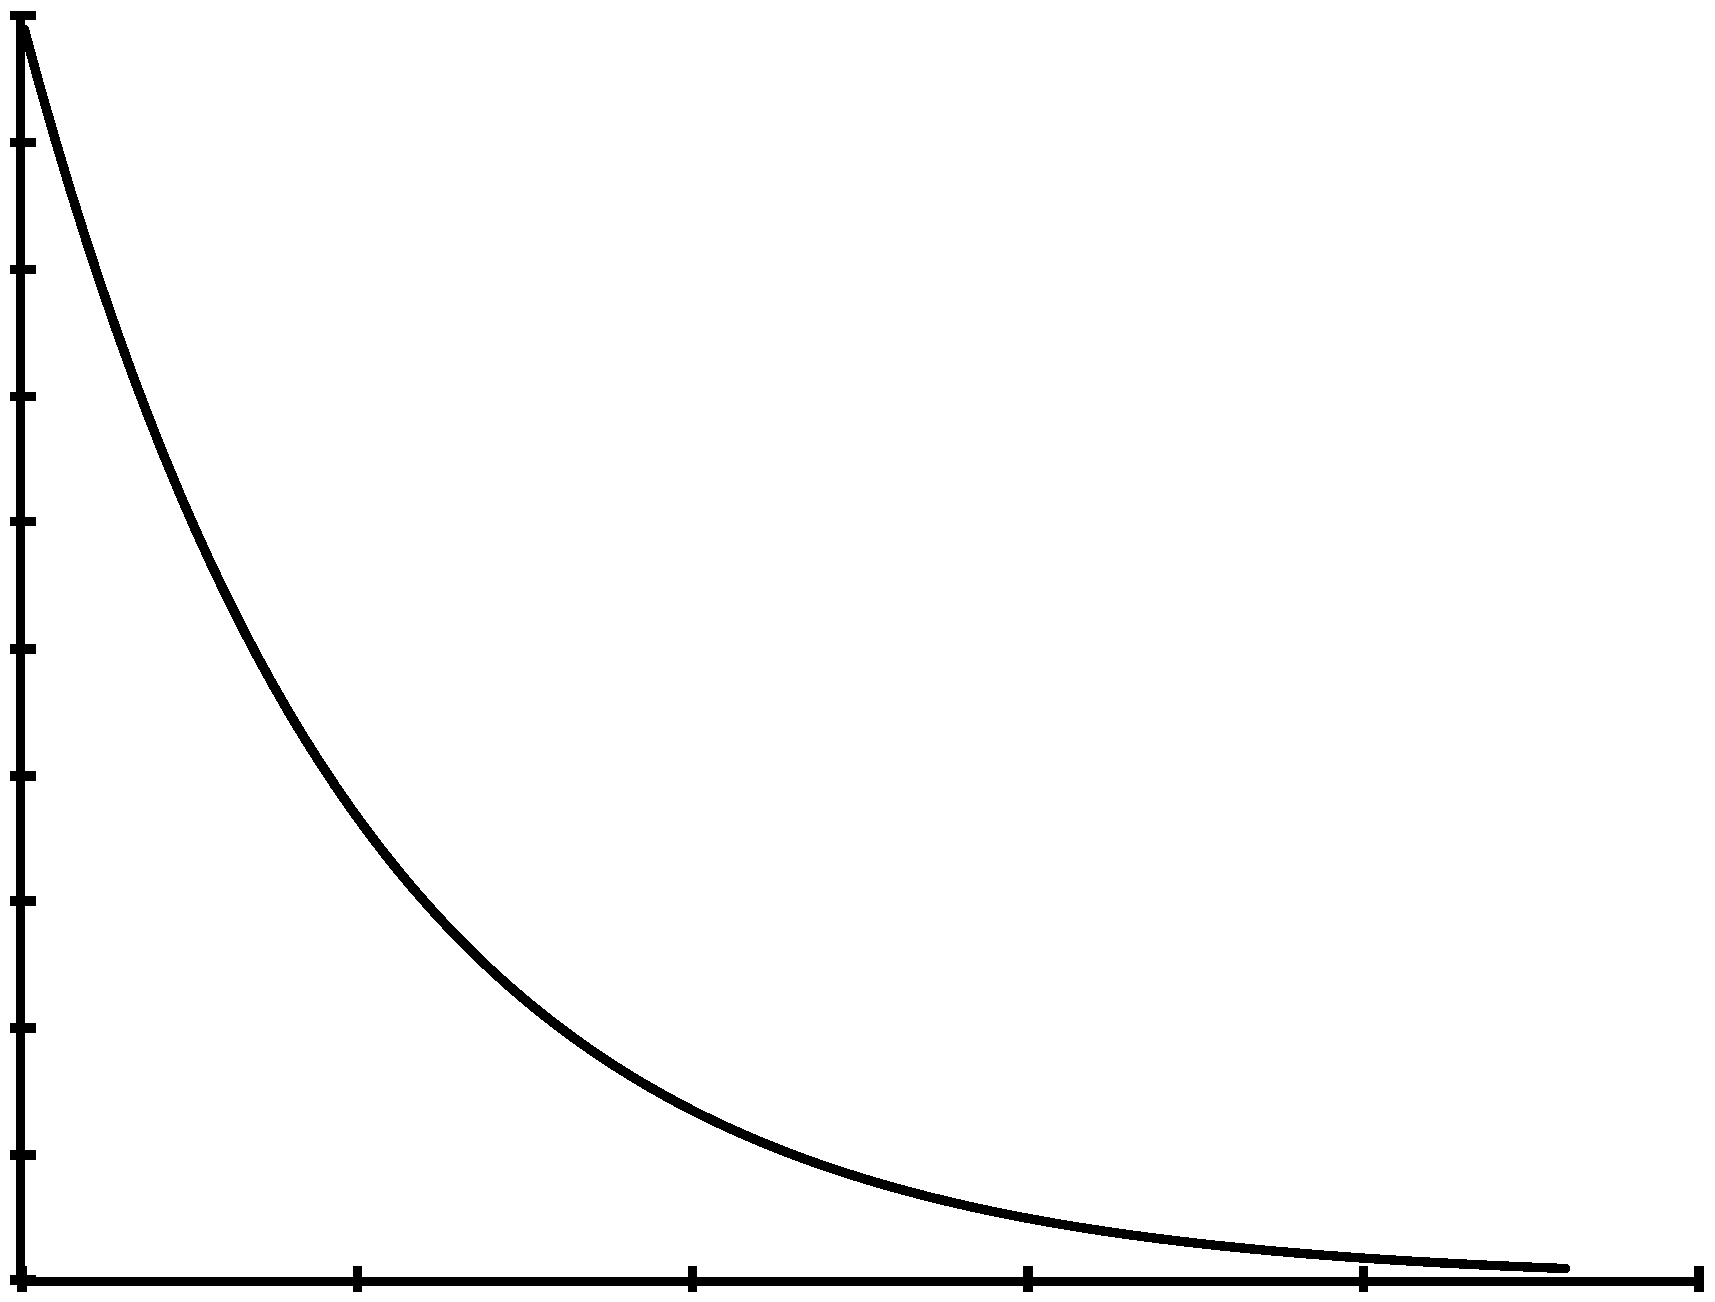
\includegraphics[width=1\textwidth]{lectModel1/expDistribution.pdf}
\end{column}
\end{columns}
\end{frame}
%***********************************************************
\begin{frame}{The Cumulative Distribution Function}

\begin{columns}[c]
\begin{column}{0.35\textwidth}
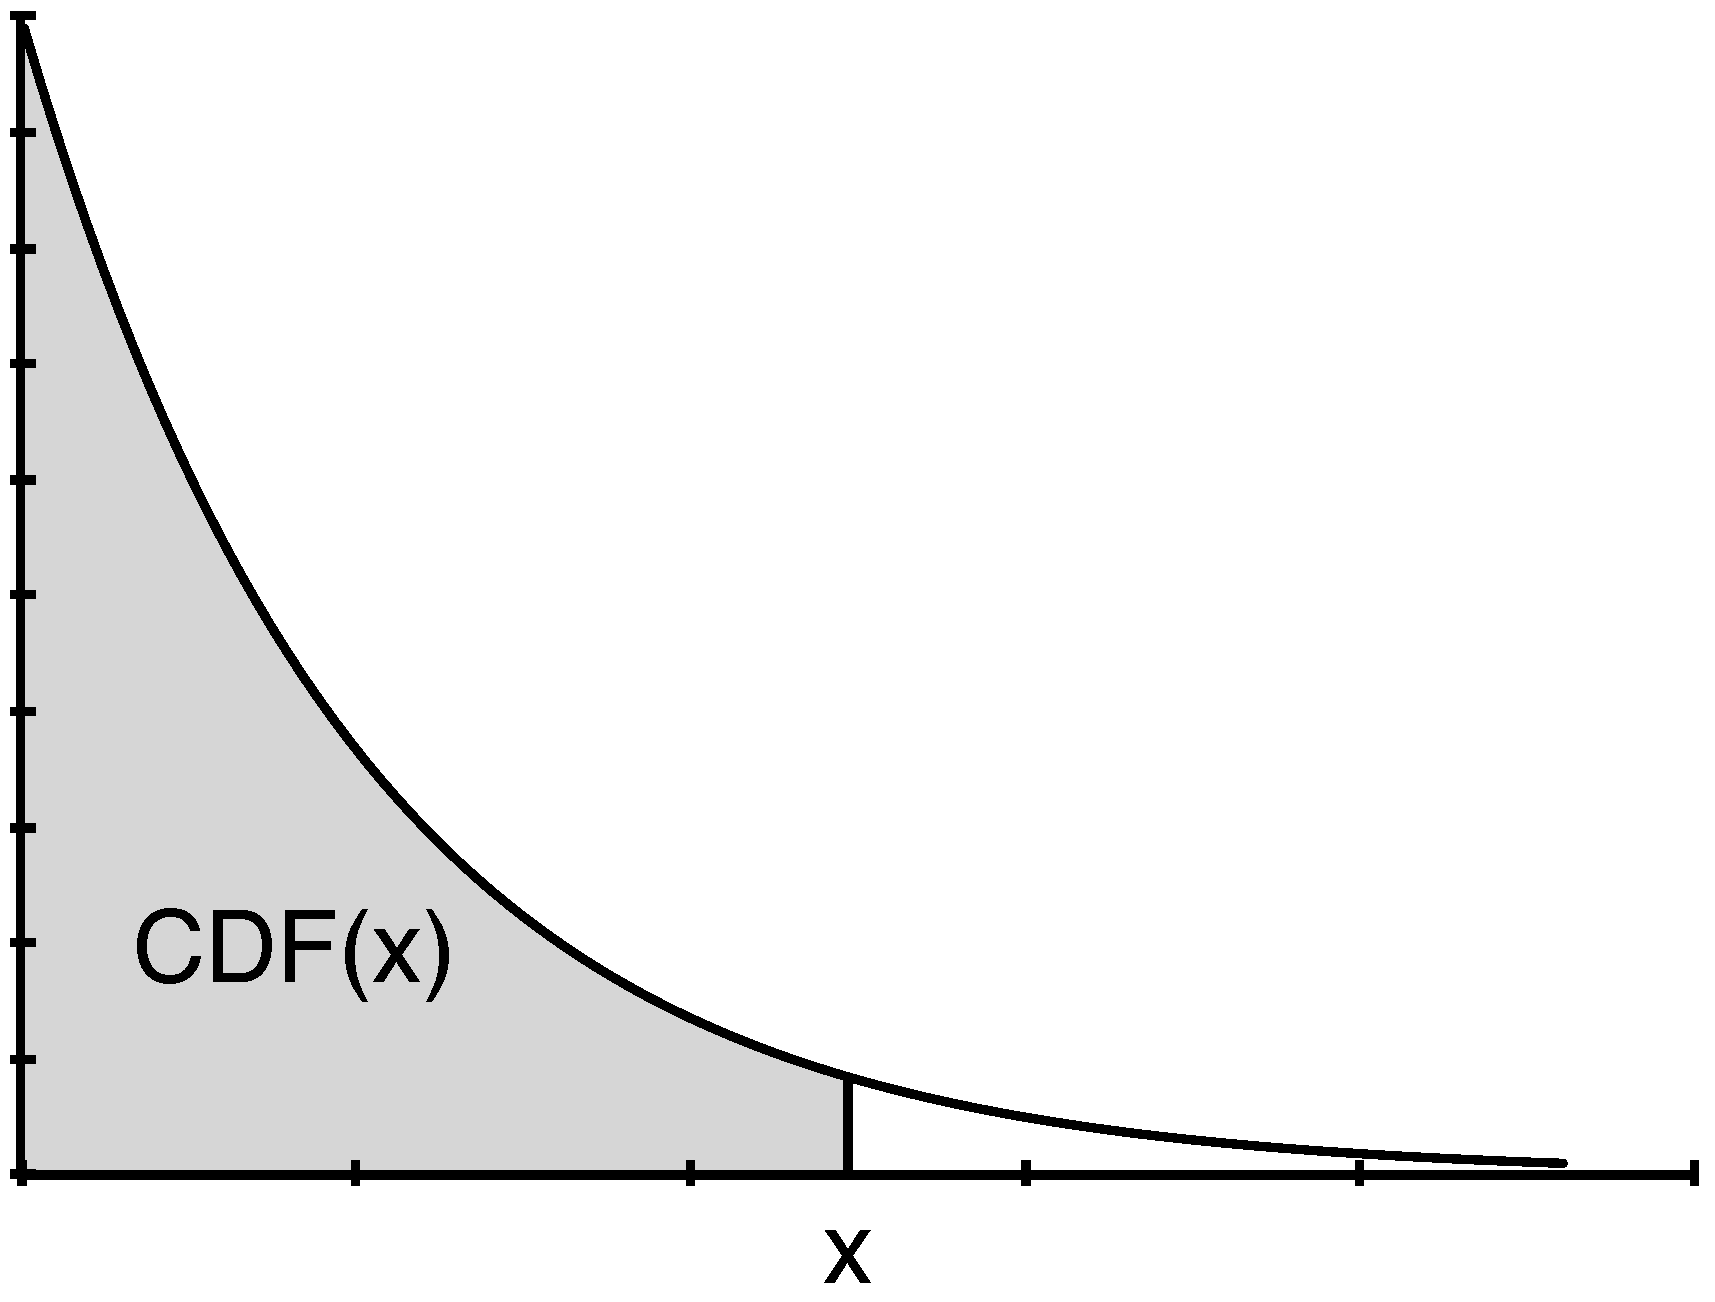
\includegraphics[width=1\textwidth]{lectModel1/expDistributionCDF.pdf}\\
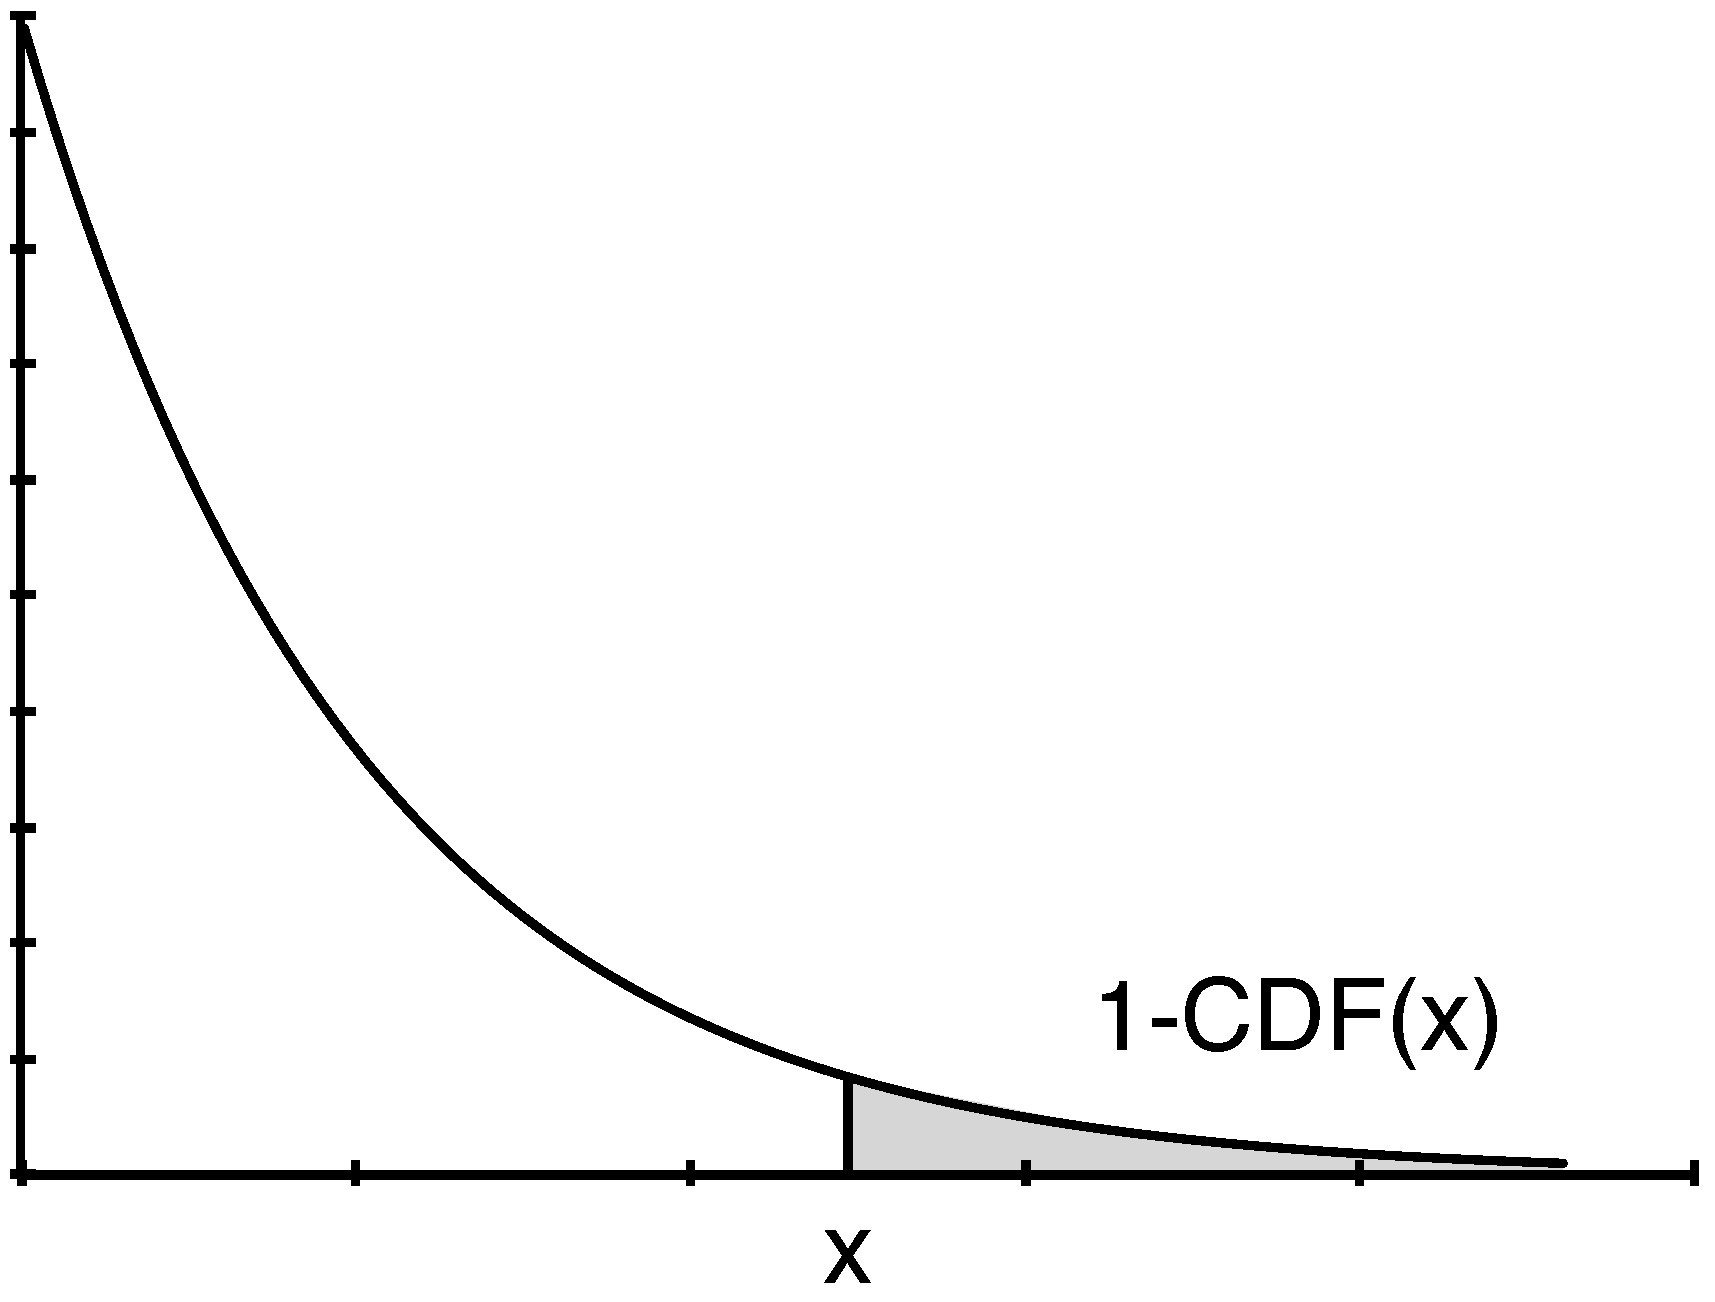
\includegraphics[width=1\textwidth]{lectModel1/expDistribution1MinusCDF.pdf}
\end{column}
\begin{column}{0.65\textwidth}
\begin{itemize}
\item The probability that the RV will have a value $\le$ x
\item Total mass at point x is the area to the left of x
\item CDF, $F_X$ of a RV $X$:
\begin{itemize}
\item $F_X(x) = P( X\le x)$
\item $F_X(b) - F_X(a) = P( a < X \le b)$
\end{itemize}
\end{itemize}
\end{column}
\end{columns}
\end{frame}


%***********************************************************
\begin{frame}{Learning the Model}

\begin{itemize}
	\item Turn in times so far at tick 100: $\{18, 22, 45, 49, 86\}$
	\begin{itemize}
	\item Know mean of exponential is $\lambda^{-1}$
	\item In our case, $44 = \lambda^{-1}$ so $\lambda \approx 0.0227$
	\item Use the CDF equation: $1 - e^{-\lambda x}$
	\vspace{1em}
	\item Recall: Want to predict how many have completed by 1 hour before due date
	\item So, $x = 167-100$
	\item CDF =  $1 - e^{-\lambda x} =  1 - e^{-0.0227 * 67}  \approx  0.781$ 
	\item So, the probability of each remaining person turning in by deadline is 0.781
	\end{itemize}
\end{itemize}
\end{frame}
%***********************************************************
\begin{frame}{The Sniff Test}

\begin{itemize}
	\item If we only look at the early finishers, we are underestimating the mean
	\item Also, we've only looked at half the students
	\item Fixing these assumptions is non-trivial - we will examine it next time
	\item If we accept our assumptions as valid $\dots$
\end{itemize}
\end{frame}

%***********************************************************
\begin{frame}{Applying the Model}

\begin{itemize}
	\item 5 people, each with 0.781 chance of turning in at deadline $- 1$ hour
	\item[?] How should we model this?
\end{itemize}


\end{frame}
%***********************************************************
\begin{frame}{Applying the Model}

\begin{itemize}
	\item 5 people, each with 0.781 chance of turning in at deadline $- 1$ hour
	\item How should we model this?
	\begin{itemize}
	\item We have a probability and two possible outcomes (Turned in by deadline or Not turned in by deadline)
	\item This looks like a good fit for the Binomial distribution
	\end{itemize}
\end{itemize}
\end{frame}

%***********************************************************
\begin{frame}{The Binomial Distribution}

\begin{columns}[c]
\begin{column}{0.6\textwidth}
\begin{itemize}
\item Is discrete
\item Has 2 parameters 
\begin{itemize}
	\item $n =$ number of independent experiments
	\item $p =$ probability of success
	\item Probability Mass Function = ${n \choose k} p^k(1-p)^{(n-k)}$
	\item Mean: $np$
	\item Variance: $np(1-p)$
	\end{itemize}
\item Good for modeling Yes/No choices, $n$ times
\item Assumes trials are independent 
\item Degenerative form is the Bernoulli distribution, when $n=1$
\end{itemize}
\end{column}
\begin{column}{0.4\textwidth}
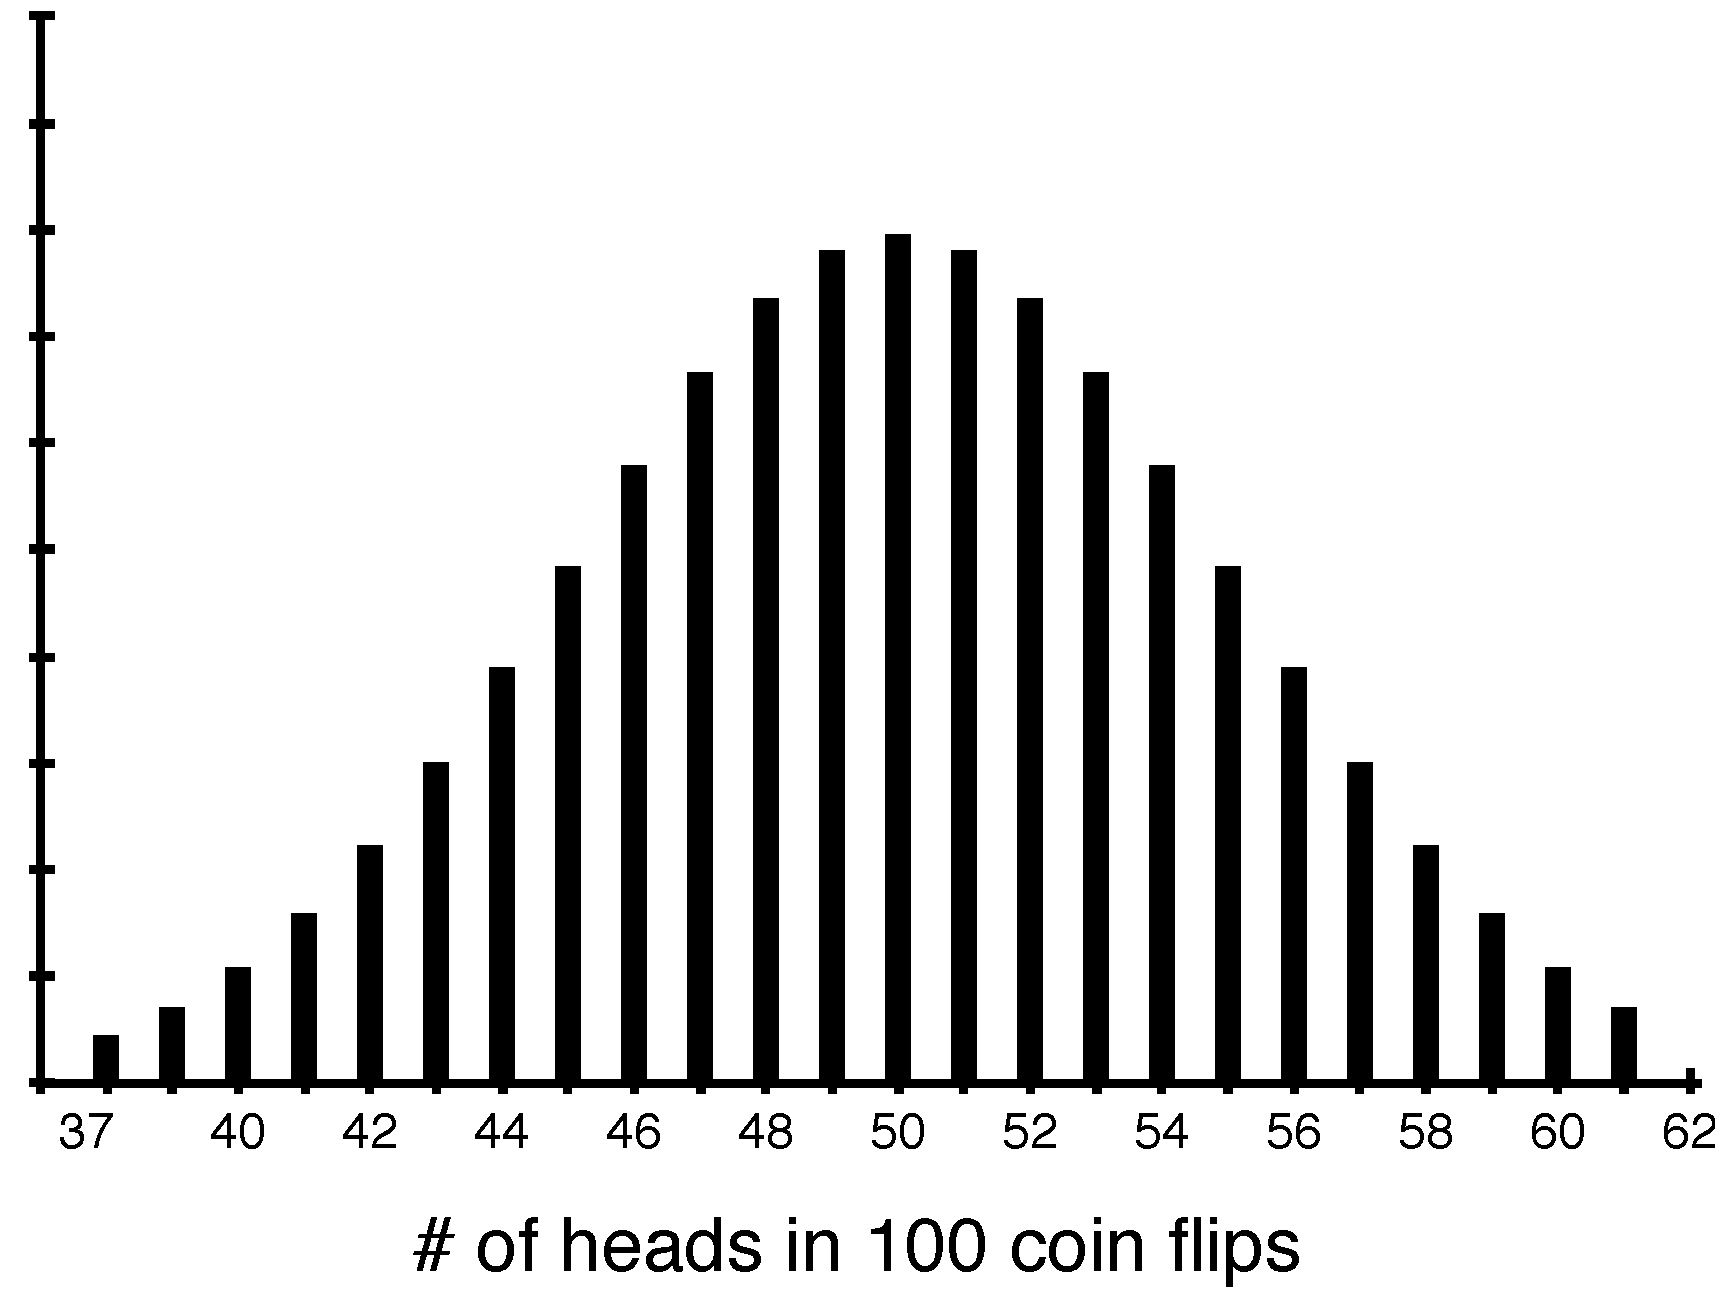
\includegraphics[width=1\textwidth]{lectModel1/binomDistribution.pdf}
\end{column}
\end{columns}
\end{frame}

%***********************************************************
\begin{frame}{The Binomial Distribution In Our Example}

\begin{columns}[c]
\begin{column}{0.6\textwidth}
\begin{itemize}
\item Think about tossing $n$ balls into a trash can
\item Each ball has a 0.781 probability of success
\item The binomial PMF and CDF will tell me probabilities of success
\item Use PMF for exact number of successes
\item Use CDF and 1-CDF for greater than or less than
\end{itemize}
\end{column}
\begin{column}{0.4\textwidth}
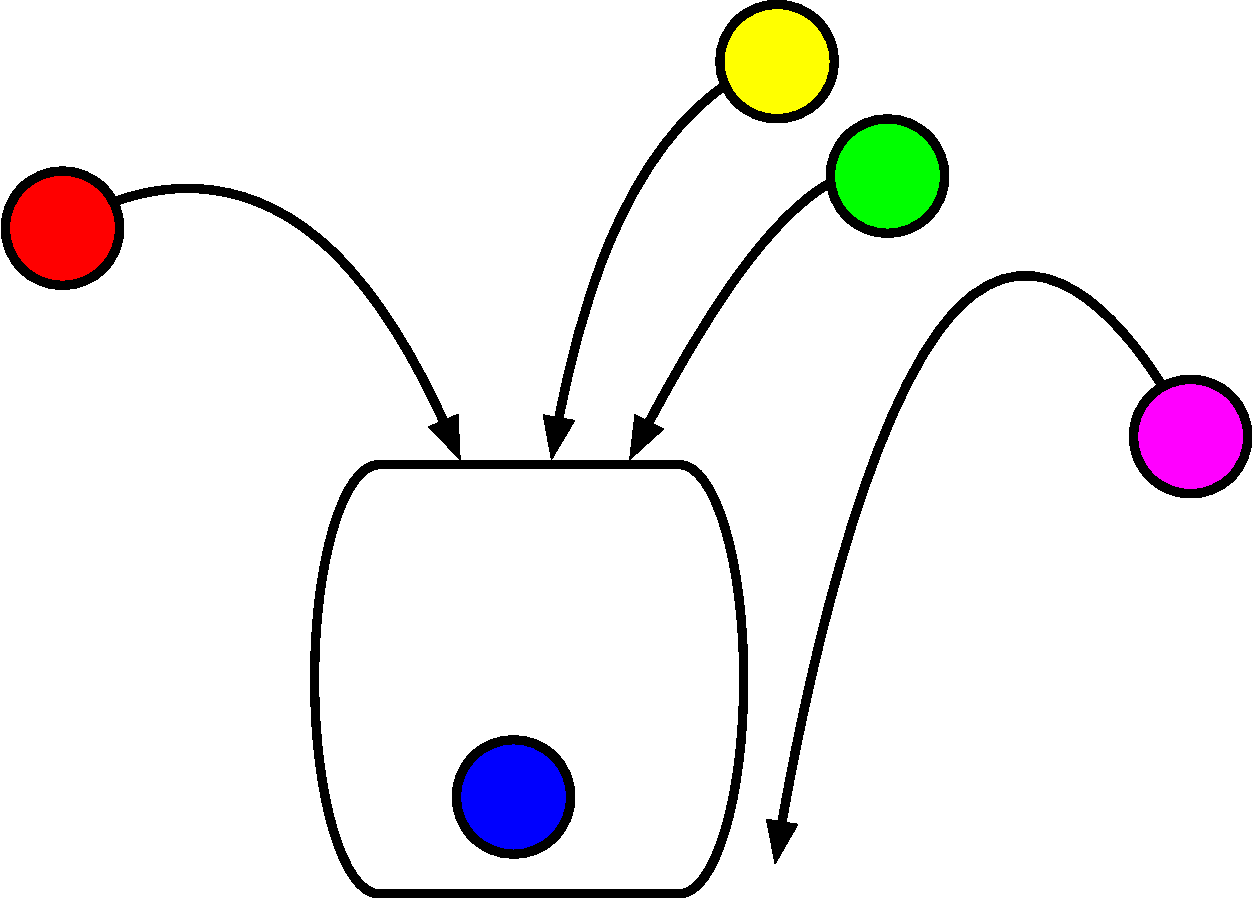
\includegraphics[width=1\textwidth]{lectModel1/ballsInTrash.pdf}
\end{column}
\end{columns}
\end{frame}


%***********************************************************
\begin{frame}{Applying the Model}

\begin{itemize}
	\item 5 people, each with 0.781 chance of turning in at deadline $- 1$ hour
	\begin{itemize}	
	\item $N \sim \textrm{Binomial (5, 0.781)}$
	\item $N$ is the number turning in assignment by the deadline
	\item Pr$(N = 5) = 0.291 = $ prob all $10$ turn in %binom.pmf(5,5,p)
	\item Pr$(N \geq 4) = 0.698 = $ prob $9+$ turn in %1 - binom.cdf(3, n, p)
	\item Pr$(N \geq 3) = 0.926 = $ prob $8+$ turn in %1 - binom.cdf(2, n, p)
	\item Pr$(N < 3) = 0.074 = $ prob $< 8$ turn in % binom.cdf(2, n, p) 
	\end{itemize}
	\item Note: there's a slight problem here
	\begin{itemize}
	\item We ignored people missing when estimating $\lambda$
	\item We will fix this next lecture!
	\end{itemize}
\end{itemize}


\end{frame}


%***********************************************************
\begin{frame}{Questions?}
\begin{itemize}
	\item[?] How can we use what we learned today?
	\vspace{2em}
	\item[?] What do we know now that we didn't know before?
\end{itemize}
\end{frame}

\end{document}
